In this section, we aim to give a concrete numerical illustration of each of the steps of the proposed framework displayed in \fref{algorithm} and applied to the example in \sref{illustrative-example}. Unless otherwise stated, the experimental setup is the same as in \sref{experimental-results} for the dual-core architecture, \ie, $\cores = 2$ in what follows. To make the explanation tractable, we simplify the UQ problem in \sref{illustrative-example} and assume that the effective channel length $\Leff$ is subjected only to the global \rv\ $\gLeff(\o)$, \ie, $\vars = 1$. As before, the nominal value $\Leff$ is 45 nm and the standard deviation is $5\%$ of 45 nm; in other words,
\[
  \Leff(\o) = \Leff + \gLeff(\o) \sim \normal\left(45 \cdot 10^{-9}, \left(2.25 \cdot 10^{-9}\right)^2\right).
\]

\step{1}{Uncertain Parameters (\sref{uncertain-parameters}).} In the scenario at hand, the transformation $\U(\o) = \oTransform{\Z(\o)}$ involves only centring and normalization of $\Leff(\o)$. Therefore,
\begin{equation} \elabel{ne-uncertain-parameters}
  \U(\o) \equiv \Leff(\o) = \oTransform{\Z(\o)} = 45 \cdot 10^{-9} (1 + 0.05 \: \Z(\o))
\end{equation}
where $\Z(\o) \sim \normal(0, 1)$.

\step{2}{Power Model (\sref{power-model}).}
Assume that, after the corresponding fitting procedure, we get the following expression for the leakage current defined in \eref{leakage-current}:
\begin{align*}
  I_\leak(\T, \Leff) = \exp(& -10.18 - 3.52 \cdot 10^8 \Leff + 0.03 \; \T \\
    & + 1.70 \cdot 10^5 \Leff \T - 3.33 \cdot 10^{-5} \T^2)
  % exp(170120.498919774.*y1.*y2-351503428.907536.*y1-3.33243035317251e-05.*y2.^2+0.0321365700019962.*y2-10.1780111244316)
\end{align*}
For instance, the formula yields a current of $1.85 \cdot 10^{-7}$~A for the nominal channel length $\Leff = 45 \cdot 10^{-9}$~nm and temperature of $45^\circ$C (\ie, $\T = 318.15$~K in the formula). Assume further that the leakage power accounts for $40\%$ of the total power at temperature of $120^\circ$C; more specifically, assume that when the dynamic power is $11.33$~W, the leakage power produced by the model is $7.56$~W. Sequentially, we compute the corresponding scaling parameter for $I_\leak$ and obtain $4.08 \cdot 10^7$; the resulting expression for the leakage model is
\begin{align*}
  \P_\leak(\T, \Leff) = 4.08 \cdot 10^7 \: \exp(& -10.18 - 3.52 \cdot 10^8 \Leff + 0.03 \; \T \\
    & + 1.70 \cdot 10^5 \Leff \T - 3.33 \cdot 10^{-5} \T^2)
\end{align*}
Finally, the power model in \eref{power-model} is
\[
  \vP(\t, \o) =
    \left(
      \begin{array}{c}
        \P_{\dyn, 1}(\t) + \P_{\leak}(\T_1(\t, \o), \oTransform{\Z(\o)}) \\
        \P_{\dyn, 2}(\t) + \P_{\leak}(\T_2(\t, \o), \oTransform{\Z(\o)})
      \end{array}
    \right)
\]
where $\P_{\dyn, i}(\t)$ and $\T_i(\t, \o)$ are the dynamic power and temperature of the $i$th processing element, respectively, and $\Leff$ is replaced by \eref{ne-uncertain-parameters}. In the equation above, it is assumed that the leakage model is the same for both processors.

\step{3}{Thermal Model (\sref{thermal-model}).} The main components of the thermal specification $\system$ of the platform are shown in \tref{hotspot}, which is a part of the default configuration of HotSpot \cite{hotspot}. Assume the two processors are placed side by side to each other and occupy a square of $16$ $\text{mm}^2$ each. As before, we utilize HotSpot to construct the equivalent RC thermal circuit of the system. The number of thermal nodes, $\nodes$, is $4 \times 2 + 12 = 20$ (see \fref{circuit}). Consequently, we obtain the matrices $\mC, \mG \in \real^{20 \times 20}$ in \eref{fourier-original} and the coefficient matrices $\mCF \in \real^{20 \times 20}, \mCS \in \real^{20 \times 2}$ in \eref{recurrence}. The discretization interval of power and temperature profiles, $\dt$, is assumed to be constant and equal to $10^{-3}$~s; therefore, the these matrices are also constant.
\begin{table}[t]
  \centering
  \caption{The thermal specification of the platform.}
  \begin{tabular}{lrc}
    \toprule
    Parameter & Value & Units \\
    \midrule
    Convection capacitance                &  140.4 & J/K \\
    Convection resistance                 &    0.1 & K/W \\
    Heat sink side                        &     60 & mm \\
    Heat sink thickness                   &    6.9 & mm \\
    Heat spreader side                    &     30 & mm \\
    Heat spreader thickness               &      1 & mm \\
    Thermal interface material thickness  &   0.02 & mm \\
    Die thickness                         &   0.15 & mm \\
    \bottomrule
  \end{tabular}
  \tlabel{hotspot}
  \vspace{-1.0em}
\end{table}


\step{4}{Surrogate Model (\sref{polynomial-chaos}).} As motivated earlier, the Hermite polynomial basis is adopted (see \tref{askey} and \fref{hermite}). Assume we decide to construct PC expansions of the total order equal to two, \ie, $\pcorder = 2$. Then, the expansion for power has the following form:
\[
  \oPC{1}{2}{\vP_k(\o)} = \pcc{\vP}_{k, 1} + \pcc{\vP}_{k, 2} \Z(\o) + \pcc{\vP}_{k, 3} (\Z(\o)^2 - 1)
\]
where $\{ 1, \Z(\o), \Z(\o)^2 - 1 \}$ is the truncated basis with three polynomials, \ie, $\pcterms = 3$ (see \eref{pc-terms}), of $\Z(\o)$. The PC expansions for temperature retain the same structure. The corresponding coefficients, $\{ \pcc{\vP}_{k, 1}, \pcc{\vP}_{k, 2}, \pcc{\vP}_{k, 3} \}$, are computed using the Gauss-Hermite quadrature as explained in \aref{gauss-quadrature}. To this end, we select the third-order quadrature rule, \ie, $\qdlevel = \qdorder = 3$, as we want it to be exact for polynomials of order at least $2 \pcorder = 4$; the rule is, in fact, exact for the fifth-order polynomials as well. The corresponding nodes and weights are displayed in \tref{quadrature} where the normalization constant of the standard Gaussian \pdf\ is taken into account. Note that the quadrature is always known and takes no computational time to be obtained. Consequently,
\begin{align*}
  \pcc{\vP}_{k, 1} = \frac{1}{\pcn_1} \oQuad{1}{1}{\vP_k(\o) \: 1} & = \frac{1}{1} \sum_{i = 1}^3 \vP_k(\qdn{\z}_i) \: \qdw_i, \\
  \pcc{\vP}_{k, 2} = \frac{1}{\pcn_2} \oQuad{1}{1}{\vP_k(\o) \: \vZ(\o)} & = \frac{1}{1} \sum_{i = 1}^3 \vP_k(\qdn{\z}_i) \: \qdn{\z}_i \: \qdw_i, \\
  \pcc{\vP}_{k, 3} = \frac{1}{\pcn_2} \oQuad{1}{1}{\vP_k(\o) \: (\vZ(\o)^2 - 1)} & = \frac{1}{2} \sum_{i = 1}^3 \vP_k(\qdn{\z}_i) \; (\qdn{\z}_i^2 - 1) \; \qdw_i
\end{align*}
where we use the shortcuts
\begin{align*}
  & \vP_k(\o) = \vP_k(\vTO_{k - 1}(\oTransform{\Z(\o)}), \oTransform{\Z(\o)}), \\
  & \vP_k(\qdn{\z}_i) = \vP_k(\vTO_{k - 1}(\oTransform{\qdn{\z}_i}), \oTransform{\qdn{\z}_i}),
\end{align*}
the nodes $\qdn{\z}_i$ and weights $\qdw_i$ are taken from \tref{quadrature}, and the normalization constants $\pcn_i$ (recall \eref{pc-coefficients}) are computed analyticaly using $\pcn_i = (i - 1)!$ \cite{ghanem1991}.

To actually perform all the computations described so far, we need a dynamic power profile $\profPdyn$; assume it is the one depicted in \fref{power}, which contains 476 power samples, \ie, $\steps = 476$. Now, for $k = 1, \dotsc, 467$, we compute the coefficients for power using the above equations and, sequentially, calculate the coefficient for temperature using \eref{pc-recurrence} and then \eref{fourier-output}.
\begin{table}[t]
  \vspace{0.5em}
  \centering
  \caption{The third-order Gauss-Hermite quadrature.}
  \begin{tabular}{lrll}
    \toprule
    Node & & Weight & \\
    \midrule
    $\qdn{\z}_1 = $ & $-1.7320508$ & $\qdw_1 = $ & $0.16666667$ \\
    $\qdn{\z}_2 = $ & $         0$ & $\qdw_2 = $ & $0.66666667$ \\
    $\qdn{\z}_3 = $ & $ 1.7320508$ & $\qdw_3 = $ & $0.16666667$ \\
    % $\qdn{\z}_1 = $ & $-1.73205080756888$ & $\qdw_1 = $ & $0.166666666666667$ \\
    % $\qdn{\z}_2 = $ & $                0$ & $\qdw_2 = $ & $0.666666666666667$ \\
    % $\qdn{\z}_3 = $ & $ 1.73205080756888$ & $\qdw_3 = $ & $0.166666666666667$ \\
    \bottomrule
  \end{tabular}
  \tlabel{quadrature}
\end{table}

\begin{figure}[t]
  \vspace{-1.0em}
  \centering
  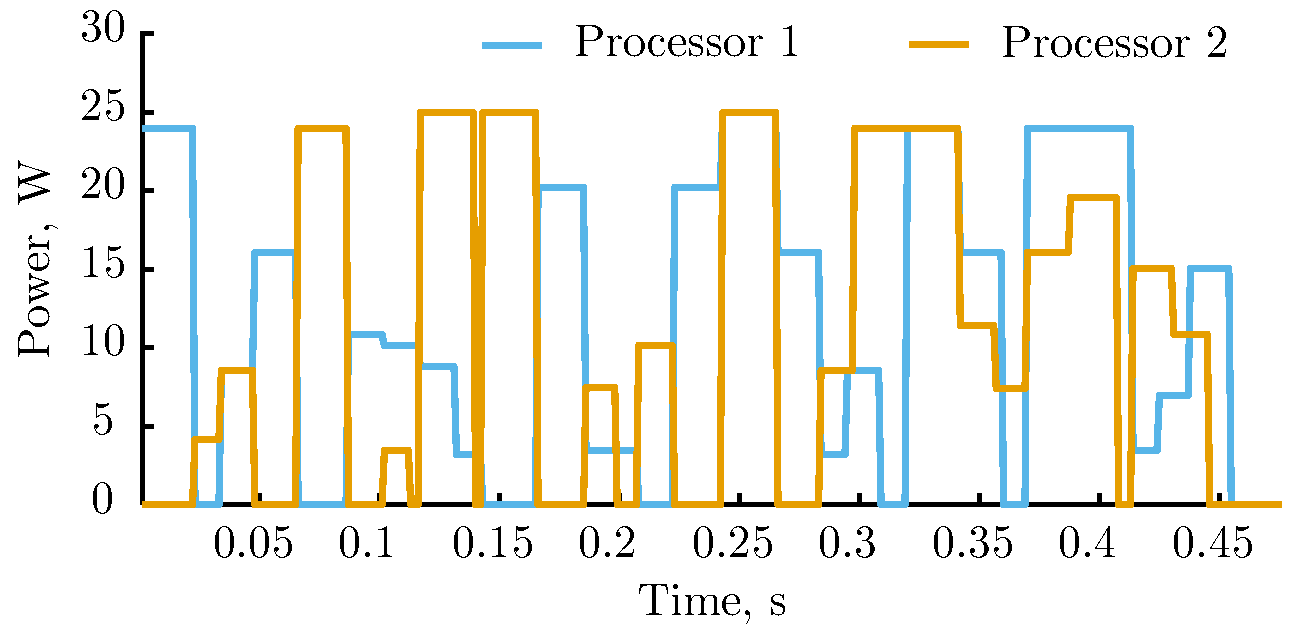
\includegraphics[width=0.90\columnwidth]{include/assets/power.pdf}
  \caption{A dynamic power profile.}
  \flabel{power}
  \vspace{-1.2em}
\end{figure}


\step{5}{Post-processing (\sref{output-processing}).}
